% Consumer's surplus under a linear demand curve
\documentclass[tikz,border=4pt]{standalone}
\renewcommand\familydefault{\sfdefault}
\usetikzlibrary{arrows.meta}
\definecolor{surplus}{RGB}{255,255,0}
\definecolor{cost}{RGB}{146,208,80}
\definecolor{callout}{RGB}{204,204,255}
\begin{document}
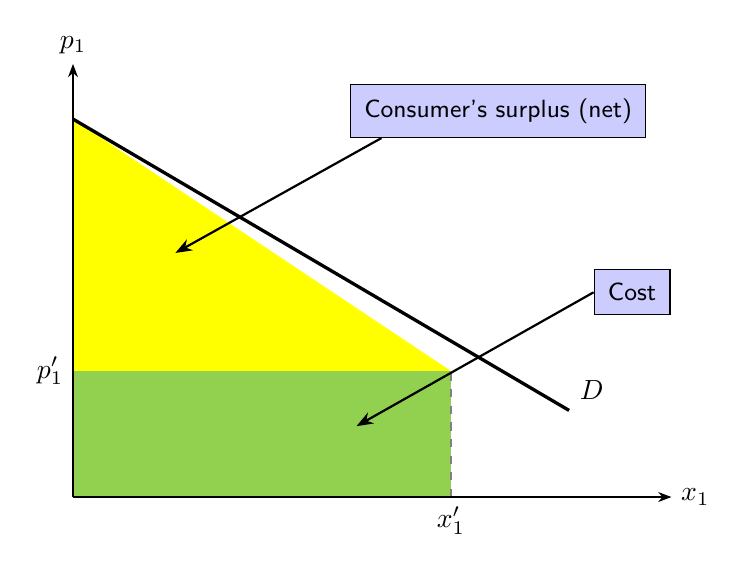
\begin{tikzpicture}[
    note/.style={draw, fill=callout, inner sep=5pt, font=\small},
    pt/.style={-{Stealth[length=6pt]}, thick}]
  % demand: from (0,4.8) through (x1'=4.8, p1'=1.6)
  \def\xa{4.8} \def\pa{1.6}
  \fill[surplus] (0,4.8) -- (\xa,\pa) -- (0,\pa) -- cycle;
  \fill[cost] (0,0) rectangle (\xa,\pa);
  \draw[gray, dashed] (\xa,0) -- (\xa,\pa);
  \draw[very thick] (0,4.8) -- (6.3,1.1) node[above right] {$D$};
  \draw[-{Stealth}] (0,0) -- (7.6,0) node[right] {$x_1$};
  \draw[-{Stealth}] (0,0) -- (0,5.5) node[above] {$p_1$};
  \node[left]  at (0,\pa) {$p_1'$};
  \node[below] at (\xa,0) {$x_1'$};
  \node[note] (cs)   at (5.4,4.9) {Consumer's surplus (net)};
  \draw[pt] (cs.south west) ++(0.4,0) -- (1.3,3.1);
  \node[note] (cost) at (7.1,2.6) {Cost};
  \draw[pt] (cost.west) -- (3.6,0.9);
\end{tikzpicture}
\end{document}
